%%%%%%%%%%%%%%%%%%%%%%%%%%%%%%%%%%%%%%%%%
% University/School Laboratory Report
% LaTeX Template
% Version 3.1 (25/3/14)
%
% This template has been downloaded from:
% http://www.LaTeXTemplates.com
%
% Original author:
% Linux and Unix Users Group at Virginia Tech Wiki 
% (https://vtluug.org/wiki/Example_LaTeX_chem_lab_report)
%
% License:
% CC BY-NC-SA 3.0 (http://creativecommons.org/licenses/by-nc-sa/3.0/)
%
%%%%%%%%%%%%%%%%%%%%%%%%%%%%%%%%%%%%%%%%%

%----------------------------------------------------------------------------------------
%	PACKAGES AND DOCUMENT CONFIGURATIONS
%----------------------------------------------------------------------------------------

\documentclass{article}

\usepackage[version=3]{mhchem} % Package for chemical equation typesetting
\usepackage{siunitx} % Provides the \SI{}{} and \si{} command for typesetting SI units
\usepackage{graphicx} % Required for the inclusion of images
\usepackage{natbib} % Required to change bibliography style to APA
\usepackage{amsmath} % Required for some math elements
\usepackage{tcolorbox} % Provide a frame around text
\usepackage{tabto}
\usepackage[normalem]{ulem}
\usepackage{listings}
\lstset{
  basicstyle=\ttfamily,
  columns=fullflexible,
  breaklines=true,
  postbreak=\mbox{\textcolor{red}{$\hookrightarrow$}\space},
}
\usepackage{geometry}
\geometry{
	left = 20mm,
	right = 20mm
}

\usepackage{french}

\setlength\parindent{0pt} % Removes all indentation from paragraphs

\renewcommand{\labelenumi}{\alph{enumi}.} % Make numbering in the enumerate environment by letter rather than number (e.g. section 6)

%\usepackage{times} % Uncomment to use the Times New Roman font

%----------------------------------------------------------------------------------------
%	DOCUMENT INFORMATION
%----------------------------------------------------------------------------------------

\title{BIG DATA \\ TP - Donn\'{e}es massives} % Title

\author{Nicolas \textsc{Lagaillardie}} % Author name

\date{\today} % Date for the report

\begin{document}

\maketitle % Insert the title, author and date

%\begin{center}
%\begin{tabular}{l r}
%Date Performed: & January 1, 2012 \\ % Date the experiment was performed
%Partners: & James Smith \\ % Partner names
%& Mary Smith \\
%Instructor: & Professor Smith % Instructor/supervisor
%\end{tabular}
%\end{center}

% If you wish to include an abstract, uncomment the lines below
% \begin{abstract}
% Abstract text
% \end{abstract}

%----------------------------------------------------------------------------------------
%	SECTION 1
%----------------------------------------------------------------------------------------

\section{Objectif}

Le but du TP est de d\'{e}terminer si le graphe (orient\'{e}) des cat\'{e}gories de Wikipedia contient des circuits. Il s’agit d’\'{e}crire un programme qui lit les donn\'{e}es et en fait une repr\'{e}sentation en m\'{e}moire, puis impl\'{e}mente l'algorithme de Tarjan.

%\begin{center}\ce{2 Mg + O2 - 2 MgO}\end{center}

% If you have more than one objective, uncomment the below:
%\begin{description}
%\item[First Objective] \hfill \\
%Objective 1 text
%\item[Second Objective] \hfill \\
%Objective 2 text
%\end{description}

\subsection{D\'{e}finitions}
\label{definitions}
\begin{description}
\item[Circuit]
Ensemble de sommets et d'ar\^{e}tes tel qu'il peut y avoir plusieurs fois le m\^{e}me sommet, mais au plus une fois la m\^{e}me ar\^{e}te.
\item[Composante fortement connect\'{e}e]
En th\'{e}orie des graphes, une composante fortement connexe d'un graphe orient\'{e} \textit{G} est un sous-graphe de \textit{G} poss\'{e}dant la propri\'{e}t\'{e} suivante, et qui est maximal pour cette propri\'{e}t\'{e} : pour tout couple \textit{(u, v)} de n\oe uds dans ce sous-graphe, il existe un chemin de \textit{u} \`{a} \textit{v}.
\item[Algorithme de Tarjan]
En th\'{e}orie des graphes, l'algorithme de Tarjan permet de d\'{e}terminer les composantes fortement connexes d'un graphe orient\'{e}. L'algorithme de Tarjan est de complexit\'{e} lin\'{e}aire, comme l'algorithme de Kosaraju, mais a l'avantage de ne faire qu'une passe sur le graphe au lieu de deux.
\end{description} 
 
%----------------------------------------------------------------------------------------
%	SECTION 2
%----------------------------------------------------------------------------------------

\section{Compr\'{e}hension des donn\'{e}es}

Trois graphes nous sont fournis, correspondant aux versions anglaise, fran\c{c}aise et espagnole de Wikip\'{e}dia. Je me suis concentr\'{e} sur la version anglaise, avant de v\'{e}rifier mon algorithme sur les autres versions.
\\*
Sur chacune de ses lignes, le premier fichier du dossier contient les arcs du graphe, et le second fichier, les noms \textit{humains} des n\oe uds. Le graphe \'{e}tant orient\'{e}, les arcs sont dirig\'{e}es du premier lien vers le second lien de chaque ligne.
\\*
Les commandes suivantes permettent de compter respectivement le nombre d'arcs et de n\oe uds dans le graphe : \\*
\begin{tcolorbox}
\begin{lstlisting}[language=sh]
$ sort enwiki-20110405-CategoryIdGraph.txt | uniq -c | wc -l
\end{lstlisting}
\begin{lstlisting}[language=sh]
$ sort enwiki-20110405-CategoryIdName.txt | uniq -c | wc -l
\end{lstlisting}
\end{tcolorbox}
~\\*
Dans ce graphe particulier, nous avons 1622626 d'arcs et 674448 n\oe uds.
 
%----------------------------------------------------------------------------------------
%	SECTION 3
%----------------------------------------------------------------------------------------

\section{Choix de la structure de donn\'{e}es et impl\'{e}mentation de l'algorithme}

J'ai impl\'{e}ment\'{e} l'ensemble de l'algorithme en \textit{Python}. Pour la structure des donn\'{e}es, j'ai construit une liste d'adjacence selon le principe suivant :

\begin{enumerate}
\begin{item}
R\'{e}cup\'{e}ration des donn\'{e}es du fichier contenant les arcs
\end{item}
\begin{item}
Pour chacune des lignes, ajouter le tuple dans un tableau \textbf{linksList} et mettre \`{a} jour l'ID maximal rencontr\'{e} \textbf{maxi}.
\end{item}
\begin{item}
R\'{e}cup\'{e}ration des donn\'{e}es du fichier contenant les n\oe uds
\end{item}
\begin{item}
Pour chacune des lignes, stocker dans l'ordre de recontre le nom \textit{humain} du n\oe ud dans un tableau \textbf{URLList}, le numéro de cette ligne \`{a} l'index [ID du n\oe ud] dans un deuxi\`{e}me tableau \textbf{indexList} et l'ID du n\oe ud dans un dernier tableau \textbf{vertices}.
\end{item}
\begin{item}
Cr\'{e}ation de la liste d'adjacence qui est un tableau \textbf{adjacentList} de taille \textit{le nombre d'\'{e}l\'{e}ments}, et qui, \`{a} chaque ID, va chercher l'index d'insertion dans \textbf{indexList} et ajouter l'ID des voisins \`{a} partir de \textbf{linksList} dans un sous tableau
\end{item}
\end{enumerate}
~\\*
Pour l'algorithme de Tarjan, j'ai suivi le pseudo-code affich\'{e} sur la page Wikip\'{e}dia qui lui est relatif.

%----------------------------------------------------------------------------------------
%	SECTION 4
%----------------------------------------------------------------------------------------

\section{R\'{e}sultats et bilan}

Voici les r\'{e}sultats obtenus, avec une moyenne de temps d'ex\'{e}cution de 10 secondes :
\\*
\begin{figure}[h]
\begin{center}
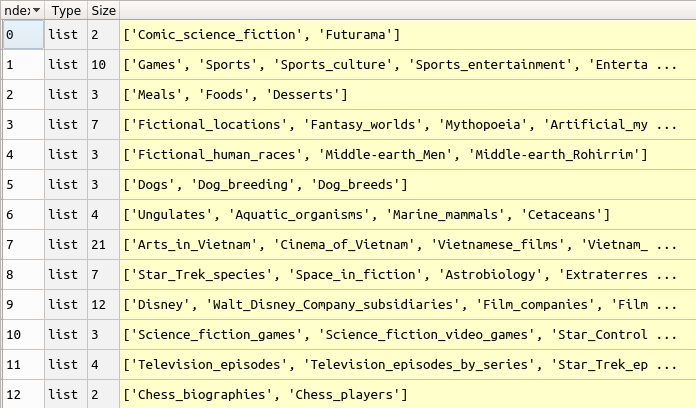
\includegraphics[width=0.64\textwidth]{consoleResultat}
\caption{R\'{e}sultats pour le Wikip\'{e}dia anglais}
\end{center}
\end{figure}
~\\*
En \'{e}tudiant les r\'{e}sultats, on se rend compte qu'il y a bien des circuits, qui sont au nombre de 378 pour le Wikip\'{e}dia anglais, et on note bien les liens \textit{humains} qu'il existe entre les diff\'{e}rentes pages d'un m\^{e}me circuit. Par exemple les \'{e}l\'{e}ments \textit{Meals}, \textit{Foods} et \textit{Desserts} font partie d'un m\^{e}me circuit, tout comme \textit{Chess\_ biographies} et \textit{Chess\_ players}. Les r\'{e}sultats semblent donc coh\'{e}rents. Par ailleurs, le temps d'ex\'{e}cution semble tr\`{e}s faible au vu de la taille des donn\'{e}es, ce qui est un avantage ind\'{e}niable. En particulier parce qu'aucune autre m\'{e}thode d'acc\'{e}l\'{e}ration n'a \'{e}t\'{e} utilis\'{e}e : GPU, multi-CPU ou autre. N\'{e}anmoins, cette dur\'{e}e d'ex\'{e}cution assez faible est obtenue au d\'{e}triment d'un important espace m\'{e}moire occup\'{e}. En effet, dans le fichier \textit{indexList}, une partie de la liste est inutilis\'{e}e puisqu'il existe moins d'\'{e}l\'{e}ments que le plus grand ID. Ainsi, une piste d'am\'{e}lioration serait de r\'{e}duire cet espace m\'{e}moire occup\'{e}, tout en contenant la dur\'{e}e d'ex\'{e}cution totale.

\end{document}